% ---------------------------------------------------------------
% Activity 2.6 - Position and speed control loop (Team 7)
% Compile:  latexmk -pdf main.tex
% Screenshots: drop the PNGs named in the grey boxes into figures/
% and rebuild; each box is replaced by the image automatically.
% ---------------------------------------------------------------
\documentclass[letterpaper, 11pt]{article}

% keep it unreal
\usepackage[top = 2cm, bottom = 2cm, left = 2cm, right = 2cm]{geometry}
\usepackage[utf8]{inputenc}          % for everything
\usepackage[english]{babel}          % language of the write-up
\usepackage[T1]{fontenc}             % fonts main
\IfFileExists{tgtermes.sty}{\usepackage{tgtermes}}{\usepackage{mathptmx}}
\usepackage{graphicx}                % images
\graphicspath{{./}{figures/}}        % path for images
\setlength{\parskip}{11pt}           % space between paragraphs

% ---- engineering content packages (math, units, tables, code) ----
\usepackage{amsmath,amssymb}
\usepackage{siunitx}
\usepackage{booktabs}
\usepackage{float}
\usepackage{caption}
\usepackage{listings}
\usepackage{enumitem}
\usepackage{xcolor}
\usepackage{tikz}
\usetikzlibrary{positioning, arrows.meta, calc}
\usepackage[hidelinks]{hyperref}
\sisetup{per-mode=symbol, exponent-product=\cdot}
\lstset{basicstyle=\ttfamily\footnotesize, numbers=left,
        numberstyle=\tiny, frame=single, breaklines=true,
        showstringspaces=false, tabsize=4, captionpos=b, language=C}

% a screenshot the team still has to add: shows a box until figures/#1 exists
\newcommand{\shot}[3]{%
  \IfFileExists{figures/#1}{\includegraphics[width=#2\linewidth]{#1}}%
  {\fcolorbox{gray}{gray!8}{\parbox[c][3.2cm][c]{#2\linewidth}{\centering\small
     \textbf{Screenshot to add:} \texttt{figures/\detokenize{#1}}\\[2pt] #3}}}}

% ---- assignment metadata ----
\newcommand{\reporttitle}{Activity 2.6}
\newcommand{\reportsubtitle}{Position and speed control loop}
\newcommand{\coursecode}{MR2006B}
\newcommand{\professor}{Federico Guedea Elizalde}

\begin{document}

\begin{titlepage}
\centering
\thispagestyle{empty}

\Large{\textsc{Instituto Tecnológico y de Estudios Superiores de Monterrey}}

\vspace{1cm}

\IfFileExists{logo.png}{
\includegraphics[scale = 0.2]{logo.png}}%
                       {\vspace{2cm}}

\bigskip

\textbf{\huge \reporttitle}

\bigskip

\textit{\Large \reportsubtitle}

\bigskip

By Team 7\\
\textbf{\Large Sondre T. Hjemgaard} \quad A01833522\\
\textbf{\Large Hakon Munch Haraldsson} \quad A01832889\\
\textbf{\Large Filip Repstad Spanne} \quad A01833674

\bigskip

Course\\
\textbf{\Large \coursecode}

Taught by\\
\textbf{\Large \professor}

\vfill

\noindent\textsc{\Large Campus Monterrey} \hfill \textsc{\Large Nuevo León}\\
\end{titlepage}

% =================================================================
\section*{Note on the measurements}

The open-loop and closed-loop tests of points 1, 7 and 14 could not be recorded on
the car. On the night the tests were planned the battery read \SI{9.4}{\volt} of
\SI{12.6}{\volt} (about \SI{3.1}{\volt} per cell, practically empty) and the labs,
where it can be charged, were closed until after the deadline. With the professor's
agreement the tests were \textbf{simulated} for this activity.

To keep the simulated tests as close to the car as possible, a \emph{virtual car}
was written (\texttt{virtual\_car.py} in \texttt{matlab/python}). It runs the firmware's own
control code (100~ms interrupt, whole encoder counts, the speed filter, the
trapezoid and \texttt{ControlPID()}) on a plant model, and writes the same telemetry
files as the real car. Its parameters are:
\begin{itemize}[nosep]
  \item dead zone $p_0 = 50\,\%$ and gain $K = \SI{1.8}{\centi\meter\per\second}$ per \%:
        taken from the feed-forward tuned by hand on the real car until it drove
        exactly \SI{1}{\meter} (offset 50\,\% PWM, \SI{0.556}{\percent} per cm/s);
  \item time constant $\tau = \SI{0.25}{\second}$: \textbf{assumed}, typical of a
        small gear-motor car; it was not measured.
\end{itemize}
Every figure that comes from the virtual car says so, and Section~7 shows how the
results change when these assumptions are wrong. The method (and all the scripts)
are the same as for real logs: only the data folder changes.

% =================================================================
\section*{1. Open-loop tests}

The car is driven without the controller using the Bluetooth command \texttt{P xx}
(motor at xx\,\% PWM), with telemetry on (\texttt{T 10}: one line every \SI{100}{\milli\second}
with time, encoder count, distance, speed, motor \%). The procedure for each test is
\texttt{T 10}, \SI{1}{\second} standing still, \texttt{P xx}, \SI{3}{\second} driving,
\texttt{X} (brake). Four steps were run: \SIlist{60;70;80;90}{\percent}.

\begin{figure}[H]
\centering
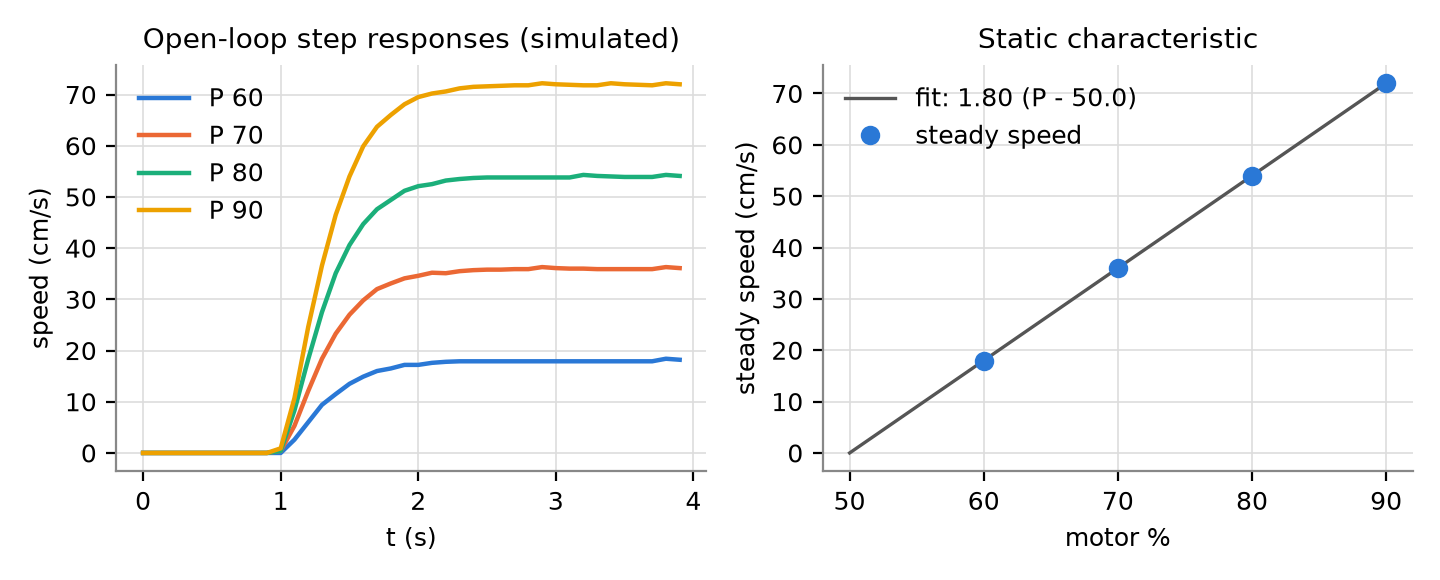
\includegraphics[width=\linewidth]{openloop_steps.png}
\caption{Open-loop step responses of the virtual car (left) and steady-state speed
against motor command (right). The speed is the firmware's filtered speed
\texttt{AverageSpeed}.}
\label{fig:ol}
\end{figure}

The steady-state speed (mean of the last second of each step) is linear in the
command above a dead zone, $v_{ss} = k\,(P - p_0)$. A least-squares line through
the four points (Figure~\ref{fig:ol}, right) gives $p_0 = 50.0\,\%$ and
$k = \SI{1.80}{\centi\meter\per\second}$ per \%, the values of the virtual car, which
checks the measurement chain. Below $p_0$ the motor torque does not overcome the
friction and the car does not move, so the plant is identified from the input
$u_p = P - p_0$.

% =================================================================
\section*{2. Identification of the model}

The four steps are resampled at $T_s = \SI{0.1}{\second}$ and merged into one
\texttt{iddata} set (input $P - p_0$ in \%, output speed in cm/s). The System
Identification Toolbox (\texttt{tfest}) fitted three structures; the same fit was
repeated in Python (least squares on the simulated response) to check it.

\begin{table}[H]
\centering
\caption{Identified models, speed (cm/s) over $P - p_0$ (\%). Fit is the normalized
root-mean-square fit of MATLAB's \texttt{compare}.}
\label{tab:models}
\begin{tabular}{@{}lll@{}}
\toprule
Structure & $G(s)$ & Fit \\
\midrule
1st order & $\dfrac{1.824}{0.387s+1}$ & 94.7\,\% \\[8pt]
1st order + dead time & $\dfrac{1.811\,e^{-0.050s}}{0.329s+1}$ & 97.7\,\% \\[8pt]
2nd order & $\dfrac{1.803}{(0.284s+1)(0.090s+1)}$ & 98.8\,\% \\
\bottomrule
\end{tabular}
\end{table}

\begin{figure}[H]
\centering
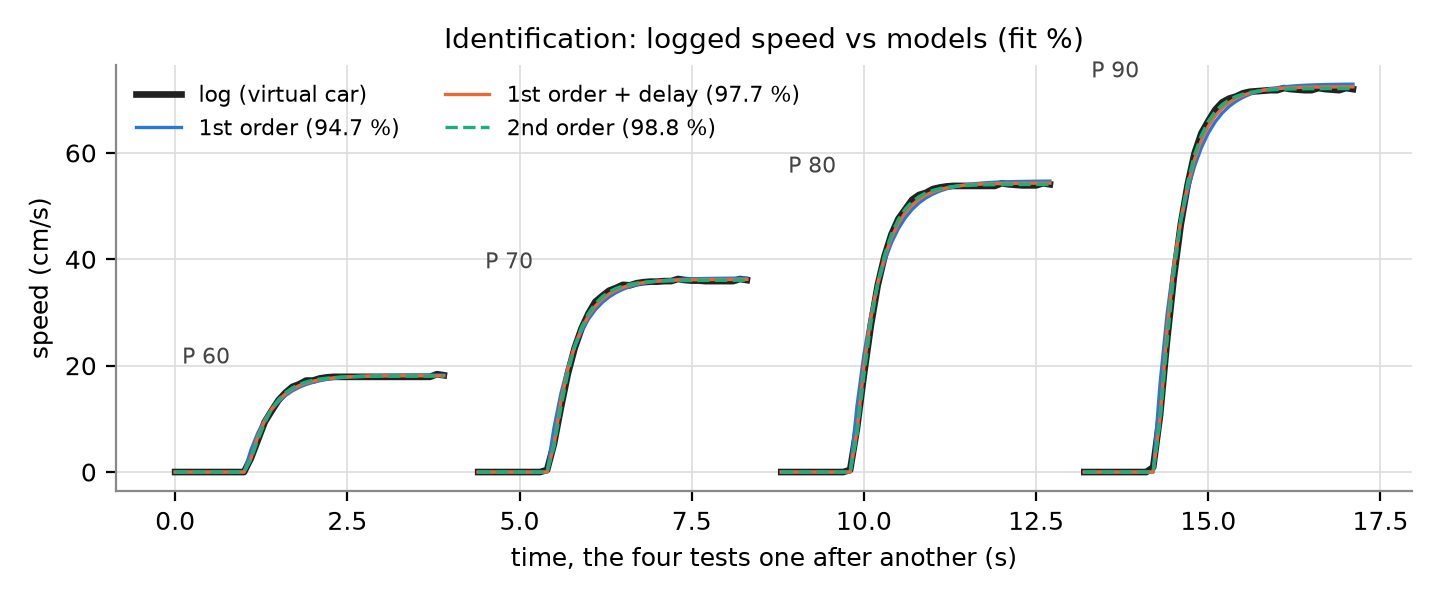
\includegraphics[width=\linewidth]{identification.png}
\caption{Logged speed of the four steps (virtual car) against the three identified
models.}
\label{fig:id}
\end{figure}

The simplest model is kept unless another one fits more than 3 points better. The
1st order + dead time model is chosen:
\[
  G(s) = \frac{V(s)}{U_p(s)} = \frac{1.811\,e^{-0.050s}}{0.329s+1}
  \quad \left[\frac{\si{\centi\meter\per\second}}{\%}\right],
  \qquad K = 1.81,\ \tau = \SI{0.33}{\second},\ L = \SI{0.05}{\second}.
\]
Identified on the 60, 80 and 90\,\% steps only, the same structure predicts the
70\,\% step with a fit of 97.8\,\%, so the model is not just following the data it
was fitted to.

The identified time constant (\SI{0.33}{\second}) is larger than the plant's
(\SI{0.25}{\second}) and a dead time appears. Both come from the speed measurement,
not from the motor: the firmware computes the speed from the counts of the last
\SI{100}{\milli\second} (an average, so on average half a period late) and then
filters it with $\bar v_k = 0.5\,\bar v_{k-1} + 0.5\,v_k$. The model therefore
describes what the controller sees, which is what the tuning needs.

\begin{figure}[H]
\centering
\shot{matlab_ident.png}{0.8}{System Identification app (\texttt{systemIdentification},
import \texttt{dat}) or the \texttt{compare} plot from \texttt{step1\_identify}}
\caption{Identification in MATLAB (\texttt{step1\_identify.m}).}
\end{figure}

% =================================================================
\section*{3. Closed loop in Simulink: sensors, actuators and target}

The car is controlled in position. The target is a distance $D$ in a total time $T$
with a trapezoidal speed profile: acceleration time $t_a$ and deceleration time $t_d$
set by the user (Bluetooth commands \texttt{tt}, \texttt{ta}, \texttt{td}). The
area under the profile is the distance, which gives the nominal speed:
\[
  D = \frac{S_n t_a}{2} + S_n (T - t_a - t_d) + \frac{S_n t_d}{2}
  \quad\Rightarrow\quad
  S_n = \frac{D}{T - (t_a + t_d)/2}.
\]
For the test run, $D = \SI{100}{\centi\meter}$, $T = \SI{8}{\second}$,
$t_a = t_d = \SI{2}{\second}$, so $S_n = 100/6 = \SI{16.7}{\centi\meter\per\second}$.
The speed profile \texttt{SP\_Vel} is used as feed-forward and its integral
\texttt{Pos\_Ref} as the position reference.

\begin{figure}[H]
\centering
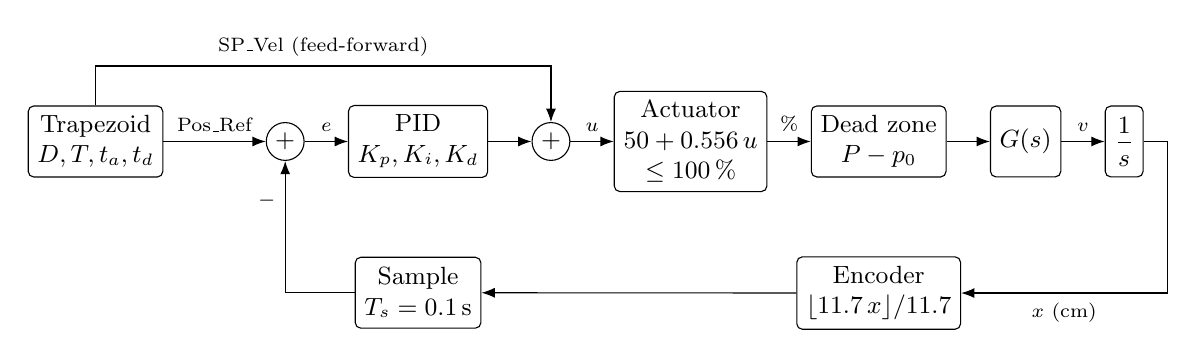
\begin{tikzpicture}[>=Latex, node distance=0.55cm and 0.55cm,
  blk/.style={draw, rounded corners=2pt, minimum height=0.9cm, align=center, font=\small},
  sum/.style={draw, circle, inner sep=1.5pt, font=\small}]
\node[blk] (ref) {Trapezoid\\$D, T, t_a, t_d$};
\node[sum, right=1.3cm of ref] (e) {$+$};
\node[blk, right=of e] (pid) {PID\\$K_p, K_i, K_d$};
\node[sum, right=of pid] (u) {$+$};
\node[blk, right=of u] (act) {Actuator\\$50 + 0.556\,u$\\$\le 100\,\%$};
\node[blk, right=of act] (dz) {Dead zone\\$P - p_0$};
\node[blk, right=of dz] (g) {$G(s)$};
\node[blk, right=of g] (int) {$\dfrac{1}{s}$};
\node[blk, below=1.0cm of dz] (enc) {Encoder\\$\lfloor 11.7\,x \rfloor / 11.7$};
\node[blk, below=1.0cm of pid] (zoh) {Sample\\$T_s = \SI{0.1}{\second}$};
\draw[->] (ref) -- node[above, font=\scriptsize]{Pos\_Ref} (e);
\draw[->] (e) -- node[above, font=\scriptsize]{$e$} (pid);
\draw[->] (pid) -- (u);
\draw[->] (ref.north) |- ++(0,0.5) -| node[above, pos=0.25, font=\scriptsize]{SP\_Vel (feed-forward)} (u.north);
\draw[->] (u) -- node[above, font=\scriptsize]{$u$} (act);
\draw[->] (act) -- node[above, font=\scriptsize]{\%} (dz);
\draw[->] (dz) -- (g);
\draw[->] (g) -- node[above, font=\scriptsize]{$v$} (int);
\draw[->] (int.east) -- ++(0.3,0) |- node[below, pos=0.75, font=\scriptsize]{$x$ (cm)} (enc);
\draw[->] (enc) -- (zoh);
\draw[->] (zoh) -| node[left, pos=0.85, font=\scriptsize]{$-$} (e);
\end{tikzpicture}
\caption{Position loop as implemented on the car and in Simulink. Units: position in
cm, speed and controller output $u$ in cm/s, actuator output in \% PWM.}
\label{fig:loop}
\end{figure}

The models of the sensors and the actuator are the ones in the firmware:
\begin{itemize}[nosep]
  \item \textbf{Actuator} (H-bridge + motor command): the controller output $u$ in
        cm/s becomes PWM through the feed-forward line found on the car,
        $P = 50 + 0.556\,u$, limited to 100\,\%; the plant then sees $P - p_0$.
  \item \textbf{Plant}: $G(s)$ from Section~2, speed in cm/s, integrated to position.
  \item \textbf{Sensor} (encoder): whole counts only, \num{1170} counts per metre
        ($c = 11.7$ counts/cm), read every $T_s$; this is a quantizer plus a sampler.
\end{itemize}
The Simulink model (\texttt{build\_simulink\_model.m}) contains two copies of this
loop, one with a continuous PID and one with the discrete PID, sampler and
quantizer, driven by the same reference.

\begin{figure}[H]
\centering
\shot{simulink_model.png}{0.9}{Diagram of \texttt{car\_position\_loop.slx}
(built by \texttt{build\_simulink\_model.m})}
\caption{Simulink model of the continuous and discrete position loops.}
\end{figure}

% =================================================================
\section*{4. Continuous PID simulation}

The PID sees the plant from its output $u$ (cm/s) to the position (cm). The constant
offsets of the actuator only move the operating point, so the linear plant is
\[
  P_c(s) = 0.556\;G(s)\,\frac{1}{s} = \frac{1.007\,e^{-0.050s}}{s\,(0.329s+1)}.
\]
The loop gain is almost exactly 1 because the feed-forward slope (0.556) is the
inverse of the plant gain (1.81): the feed-forward alone already drives the car at
the right speed, and the PID only has to correct the error. Figure~\ref{fig:cd}
shows the timed run with the continuous PI tuned in Section~6 (blue).

\begin{figure}[H]
\centering
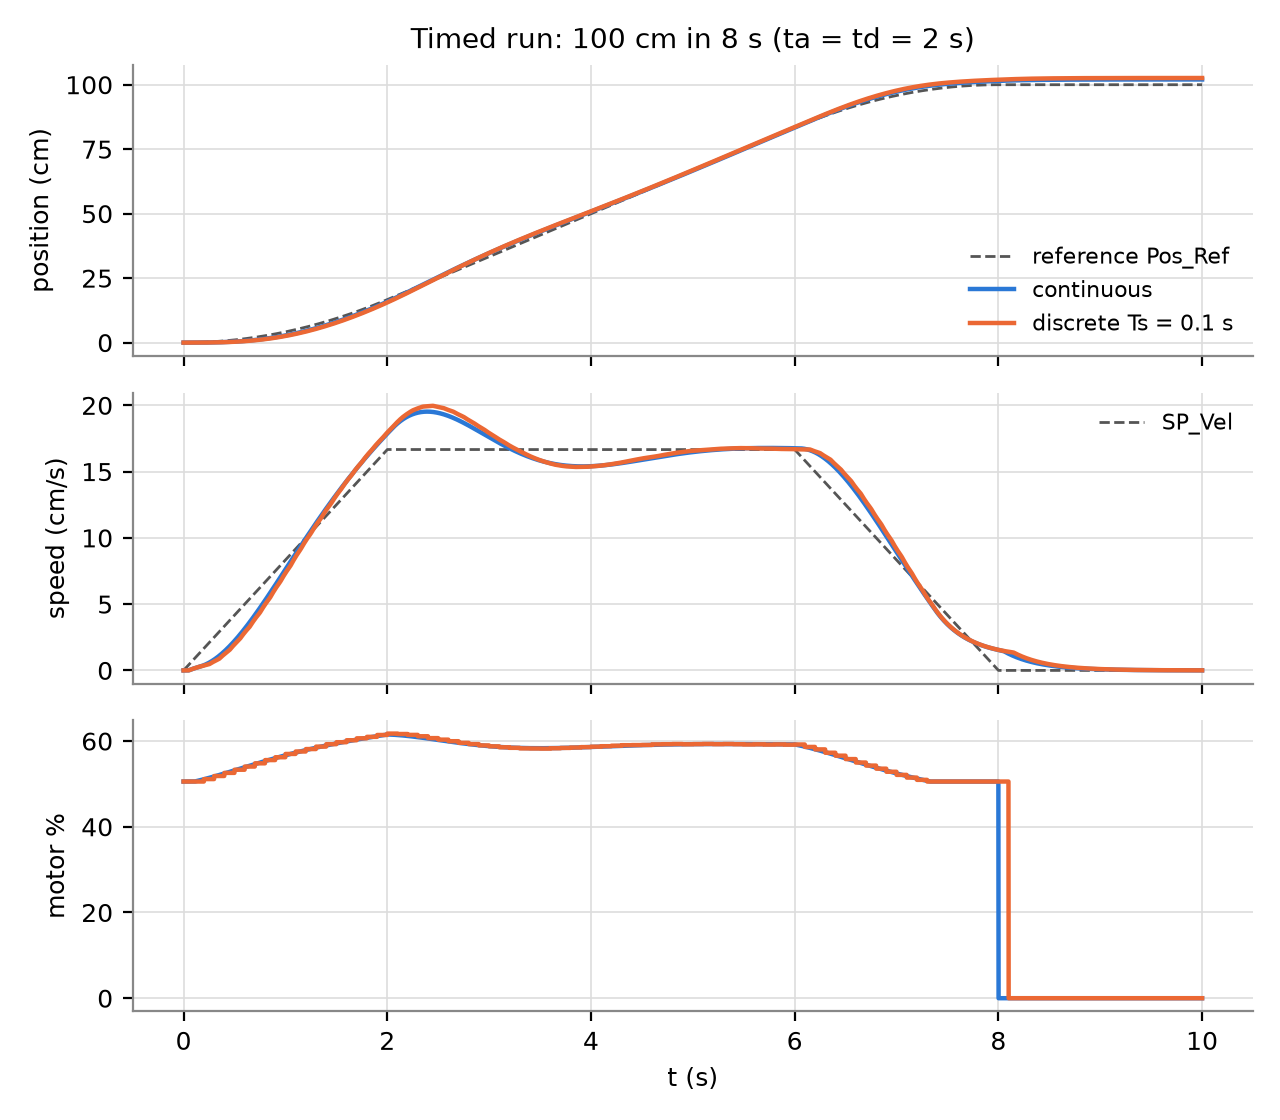
\includegraphics[width=0.9\linewidth]{cont_vs_disc.png}
\caption{Simulated timed run, \SI{100}{\centi\meter} in \SI{8}{\second}: continuous
PI ($K_p = 2.04$, $K_i = 1.25$) and discrete PI at $T_s = \SI{0.1}{\second}$
($K_p = 2.06$, $K_i = 0.90$).}
\label{fig:cd}
\end{figure}

% =================================================================
\section*{5. Discretization and sampling time}

The discrete loop samples the encoder and updates the motor every $T_s$, with the
plant seen through a zero-order hold, $P_d(z) = \mathcal{Z}\{\text{ZOH}\cdot P_c(s)\}$
(\texttt{c2d(Pc, Ts, 'zoh')}). The PID is discretized exactly as \texttt{ControlPID()}
computes it, backward Euler for both the integral and the derivative:
\[
  C(z) = K_p + K_i\,\frac{T_s\,z}{z-1} + K_d\,\frac{z-1}{T_s\,z}.
\]

Three arguments fix $T_s = \SI{0.1}{\second}$:
\begin{itemize}[nosep]
  \item \textbf{Bandwidth.} The tuned continuous loop has a closed-loop bandwidth of
        \SI{3.26}{\radian\per\second}. Sampling at $\omega_s = 2\pi/T_s =
        \SI{62.8}{\radian\per\second}$ is 19 times faster, inside the usual
        10--30 times.
  \item \textbf{Encoder resolution.} At the cruise speed of \SI{16.7}{\centi\meter\per\second}
        the car advances $16.7 \cdot 11.7 \cdot T_s = 19.5$ counts per period at
        $T_s = \SI{0.1}{\second}$, so the speed is known to one count in 20 (5\,\%). At
        \SI{0.02}{\second} it would be 4 counts and a resolution of 26\,\%.
  \item \textbf{Simulation} (Table~\ref{tab:ts}, Figure~\ref{fig:ts}): the same gains
        at different $T_s$. Going from \SI{0.02}{\second} to \SI{0.1}{\second} adds
        only \SI{0.14}{\centi\meter} of RMS error; above \SI{0.2}{\second} it grows
        quickly.
\end{itemize}

\begin{table}[H]
\centering
\caption{Tracking error of the timed run for different sampling times (discrete PI,
$K_p = 2.06$, $K_i = 0.90$). Final error: negative means the car stops past
\SI{100}{\centi\meter}.}
\label{tab:ts}
\begin{tabular}{@{}cccc@{}}
\toprule
$T_s$ (s) & RMS error (cm) & Max error (cm) & Final error (cm) \\
\midrule
continuous & 0.97 & 1.53 & $-2.0$ \\
0.02 & 1.04 & 1.74 & $-2.3$ \\
0.05 & 1.09 & 1.82 & $-2.4$ \\
\textbf{0.10} & \textbf{1.18} & \textbf{1.97} & $\mathbf{-2.6}$ \\
0.20 & 1.37 & 2.28 & $-3.0$ \\
0.40 & 1.89 & 3.02 & $-3.9$ \\
\bottomrule
\end{tabular}
\end{table}

\begin{figure}[H]
\centering
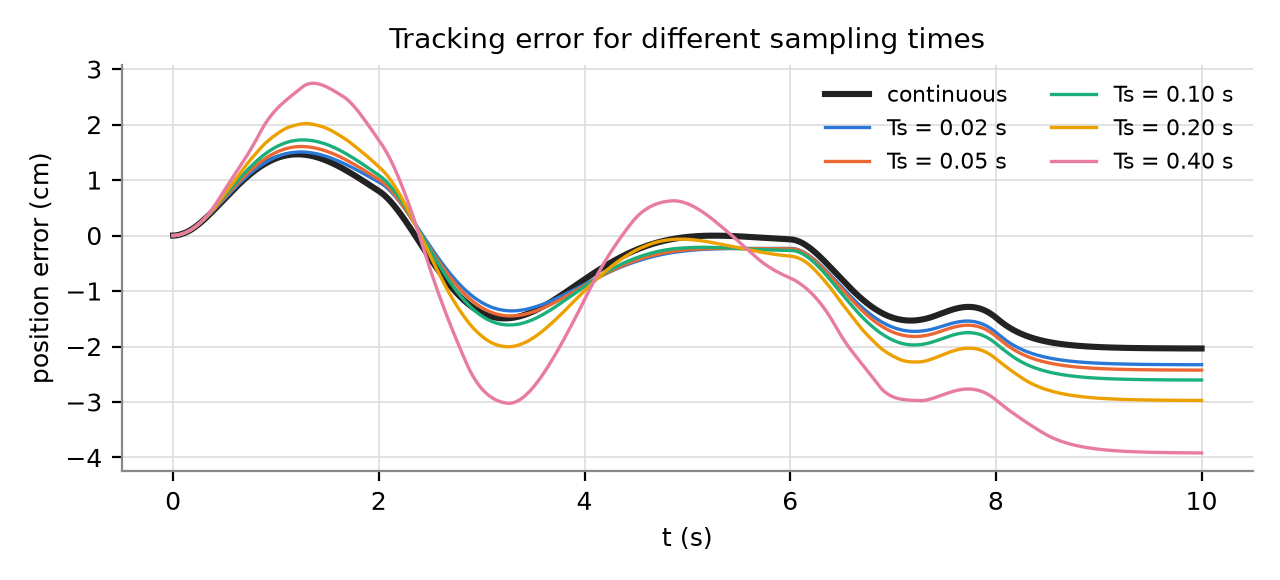
\includegraphics[width=0.85\linewidth]{ts_sweep.png}
\caption{Position error during the run for different sampling times.}
\label{fig:ts}
\end{figure}

% =================================================================
\section*{6. Tuning of the discrete PID}

The PI gains are found with \texttt{pidtune} on $P_d(z)$ for a target phase margin
and crossover frequency. For a PI, the crossover $\omega_c$ and the phase margin
fix both gains: at $\omega_c$, $C(e^{j\omega_c T_s})\,P_d(e^{j\omega_c T_s})$ must
have magnitude 1 and phase $-180^\circ + \text{PM}$. The phase margin was chosen by
simulating the timed run for each target, both on the identified model and with the
dead zone off by $\pm 5\,\%$ and the gain off by $\pm 20\,\%$ (worst case of nine
combinations). The crossover is the one with the smallest worst-case error.

\begin{table}[H]
\centering
\caption{Discrete PI for different phase-margin targets. RMS error of the timed run,
nominal and worst of the nine mismatch cases.}
\label{tab:pm}
\begin{tabular}{@{}lcccccc@{}}
\toprule
Design & $\omega_c$ (rad/s) & $K_p$ & $K_i$ & GM (dB) & RMS nominal (cm) & RMS worst (cm) \\
\midrule
PM $30^\circ$ & 2.10 & 2.41 & 1.23 & 10.9 & 1.01 & 2.87 \\
\textbf{PM $\mathbf{35^\circ}$} & \textbf{1.85} & \textbf{2.06} & \textbf{0.90} & \textbf{12.5} & \textbf{1.18} & \textbf{3.14} \\
PM $45^\circ$ & 1.55 & 1.69 & 0.42 & 15.0 & 1.43 & 4.35 \\
PM $60^\circ$ & 1.20 & 1.28 & 0.04 & 18.2 & 1.65 & 8.80 \\
\midrule
Hand-tuned on the car (PM $19^\circ$) & 2.90 & 3.80 & 2.50 & 7.3 & 0.59 & 2.66 \\
\bottomrule
\end{tabular}
\end{table}

The usual target of $60^\circ$ does not work here: the plant already has
$-90^\circ$ from the integrator plus the lag of $\tau$, the dead time and the
sampling, so $60^\circ$ is only reachable at a low crossover, where the integral
gain drops to almost zero and the worst-case error is three times larger.
$35^\circ$ is the compromise, with a gain margin of \SI{12.5}{\decibel}:
\[
  \text{continuous: } K_p = 2.04,\ K_i = 1.25; \qquad
  \text{discrete } (T_s = \SI{0.1}{\second})\text{: } K_p = 2.06,\ K_i = 0.90,\ K_d = 0.
\]
The discrete $K_i$ is lower than the continuous one because the sample and hold adds
about $\omega_c T_s/2 = 5^\circ$ of lag at the crossover, which the PI makes up for
with less integral phase lag. $K_d$ was left at zero: the timed run has no sudden
reference changes and the derivative of a 20-count signal is noisy.

\begin{figure}[H]
\centering
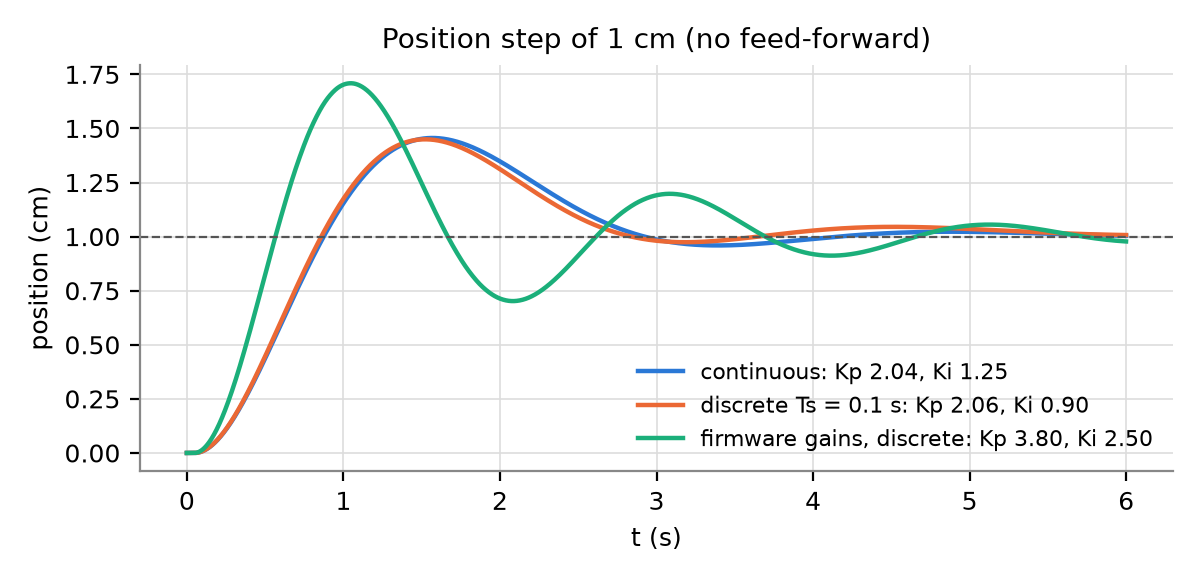
\includegraphics[width=0.75\linewidth]{step_response.png}
\caption{Response to a \SI{1}{\centi\meter} position step without feed-forward
(the worst case for the PID alone).}
\label{fig:step}
\end{figure}

\begin{figure}[H]
\centering
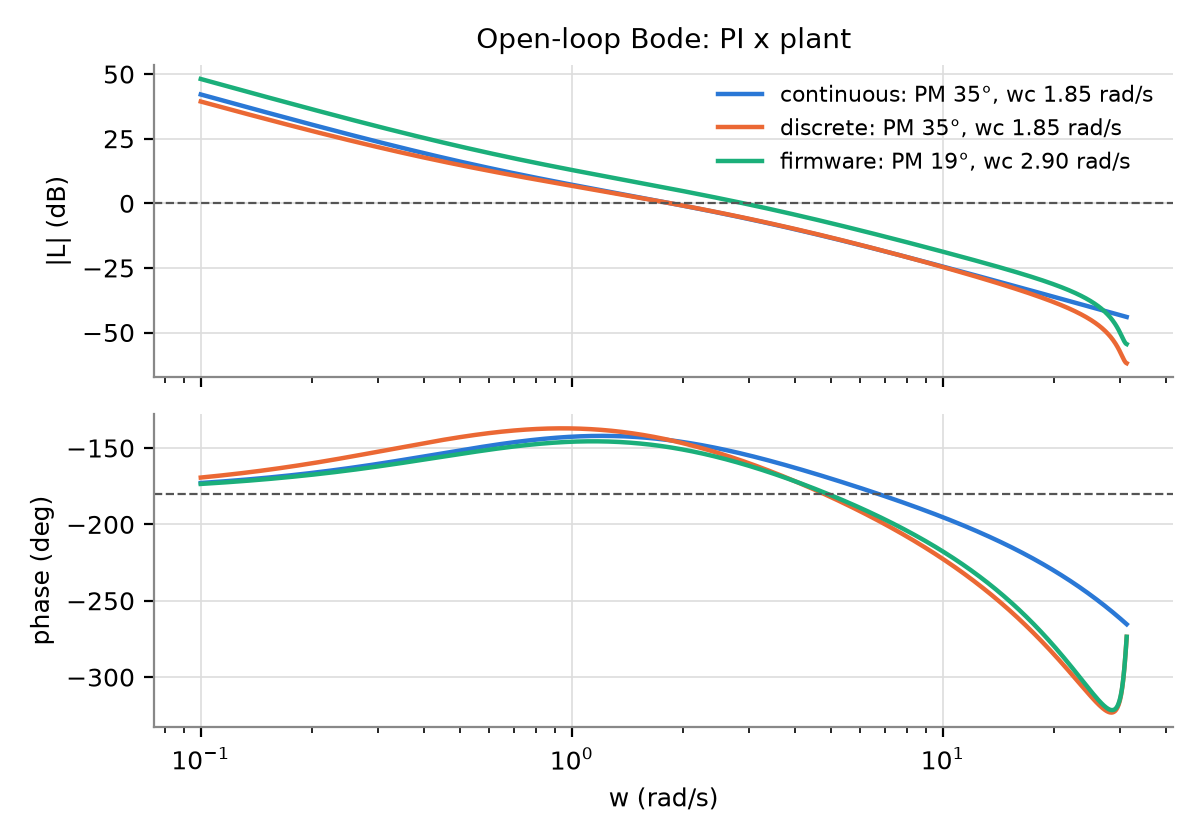
\includegraphics[width=0.75\linewidth]{bode.png}
\caption{Open-loop Bode diagram, $C \cdot P$, with phase margins and crossovers.}
\label{fig:bode}
\end{figure}

% =================================================================
\section*{7. Validation of the simulation}

The simulation was checked in three ways.

\textbf{Model.} The model predicts a step that was not used to fit it with 97.8\,\%
fit (Section~2).

\textbf{Closed loop.} A timed run (\texttt{tt 8}, \texttt{ta 2}, \texttt{td 2},
\texttt{d1}, gains $K_p = 3.8$, $K_i = 2.5$, $K_d = 0.05$) was logged from the virtual
car and compared with the discrete simulation of Section~5 (\texttt{step4\_validate.m}),
Figure~\ref{fig:val}. The two positions differ by \SI{0.55}{\centi\meter} RMS; the
car stops at \SI{100.8}{\centi\meter} and the simulation at \SI{101.0}{\centi\meter}.
The speed in the simulation leads the logged \texttt{AverageSpeed} slightly,
because the log contains the filter delay that the model represents with a dead time.

\begin{figure}[H]
\centering
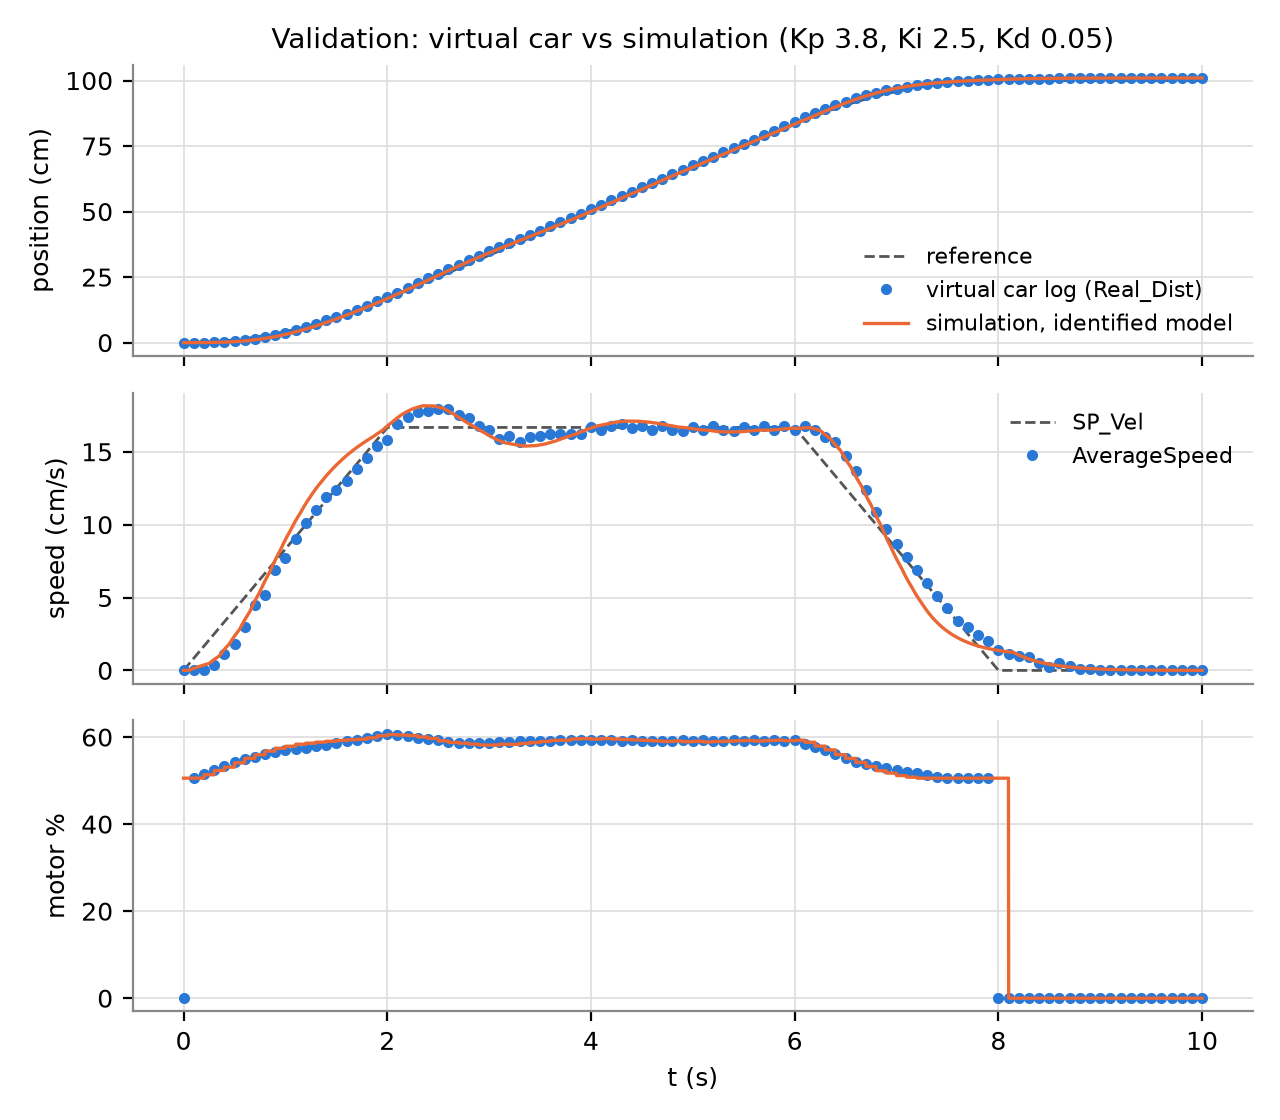
\includegraphics[width=0.85\linewidth]{validation.png}
\caption{Validation: logged run of the virtual car against the discrete simulation
with the identified model.}
\label{fig:val}
\end{figure}

\textbf{Robustness to the assumptions.} The virtual car's $\tau$ was assumed and its
$p_0$ and $K$ were derived from the feed-forward, so the timed run was repeated on
the virtual car with each parameter changed (Table~\ref{tab:sens}).

\begin{table}[H]
\centering
\caption{Timed run of \SI{100}{\centi\meter} on the virtual car when its parameters
differ from the assumptions: final position and RMS tracking error.}
\label{tab:sens}
\begin{tabular}{@{}lcccc@{}}
\toprule
& \multicolumn{2}{c}{Tuned PI (2.06, 0.90)} & \multicolumn{2}{c}{Hand-tuned (3.8, 2.5, 0.05)} \\
\cmidrule(lr){2-3}\cmidrule(l){4-5}
Virtual car & Final (cm) & RMS (cm) & Final (cm) & RMS (cm) \\
\midrule
As assumed & 101.7 & 0.86 & 100.8 & 0.43 \\
$\tau = \SI{0.10}{\second}$ & 100.9 & 0.46 & 100.5 & 0.23 \\
$\tau = \SI{0.50}{\second}$ & 104.8 & 1.74 & 102.9 & 0.90 \\
$p_0 = 45\,\%$ & 110.9 & 2.10 & 110.3 & 1.47 \\
$p_0 = 55\,\%$ & 101.2 & 2.18 & 100.4 & 1.05 \\
$K - 20\,\%$ & 103.1 & 1.36 & 101.5 & 0.69 \\
$K + 20\,\%$ & 100.8 & 0.84 & 100.5 & 0.40 \\
\bottomrule
\end{tabular}
\end{table}

Both gain sets stay stable in every case. The one large error, $p_0 = 45\,\%$,
is a limitation of the firmware rather than of the gains: during a run the command
is never below \SI{1}{\centi\meter\per\second}, i.e.\ 50.6\,\% PWM, and a car that
already moves at 45\,\% cannot slow down enough during the deceleration. On the real
car this would show as an overshoot of the target; the fix would be to allow a
lower command, or to brake, at the end of the run.

% =================================================================
\section*{8. Sensors and actuators}

\begin{table}[H]
\centering
\caption{Sensors and actuators used for the control and status of the car.}
\label{tab:dev}
\begin{tabular}{@{}lll@{}}
\toprule
Device & Role & Interface \\
\midrule
DC gear motor + L298N H-bridge & Actuator: drives the car & PWM (TIM1) + 2 GPIO \\
Quadrature hall encoder on the motor & Sensor: position and speed & Encoder mode (TIM5) \\
HC-SR04 ultrasonic sensor & Sensor: obstacle distance & GPIO trigger + EXTI echo \\
Bluetooth module (HC-05 type) & Commands and telemetry & USART1, \SI{9600}{baud} \\
SSD1306 OLED display $128\times64$ & Internal status & I2C1 \\
Steering servo & Actuator: steering (not in the loop) & PWM (TIM2) \\
Battery divider 10k/3.3k & Battery voltage & ADC1 \\
\bottomrule
\end{tabular}
\end{table}

% =================================================================
\section*{9. Connections}

Figure~\ref{fig:wiring} shows how the devices are connected to the NUCLEO-F446RE.
The HC-SR04 echo is a \SI{5}{\volt} signal, so it passes through a 1k/2k divider
to \SI{3.3}{\volt} before PA7. The board is powered from the car (jumper JP5 on
E5V); the USB cable is only for programming and the virtual COM port.

\begin{figure}[H]
\centering
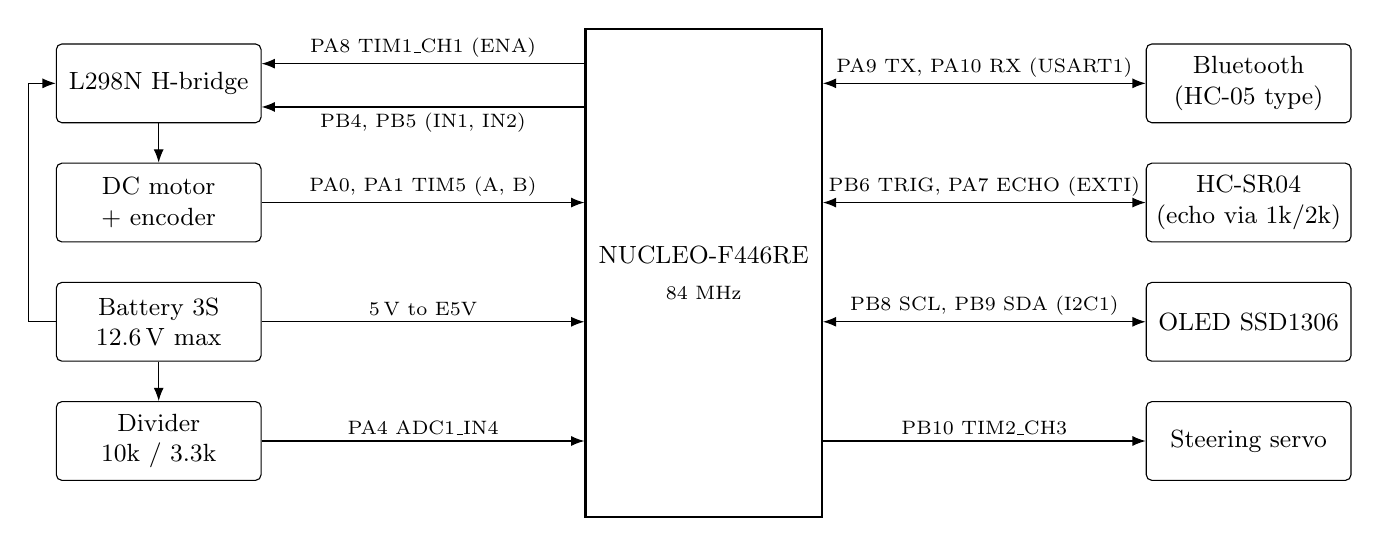
\begin{tikzpicture}[>=Latex, font=\small,
  dev/.style={draw, rounded corners=2pt, minimum width=2.6cm, minimum height=1cm, align=center},
  lab/.style={font=\scriptsize, above, inner sep=2pt}]
\node[draw, thick, minimum width=3.0cm, minimum height=6.2cm, align=center] (mcu) {NUCLEO-F446RE\\[2pt]\scriptsize 84 MHz};
\node[dev, left=4.1cm of mcu.north west, anchor=north east, yshift=-0.2cm] (hb) {L298N H-bridge};
\node[dev, below=0.5cm of hb] (mot) {DC motor\\+ encoder};
\node[dev, below=0.5cm of mot] (bat) {Battery 3S\\\SI{12.6}{\volt} max};
\node[dev, below=0.5cm of bat] (div) {Divider\\10k / 3.3k};
\node[dev, right=4.1cm of mcu.north east, anchor=north west, yshift=-0.2cm] (bt) {Bluetooth\\(HC-05 type)};
\node[dev, below=0.5cm of bt] (us) {HC-SR04\\(echo via 1k/2k)};
\node[dev, below=0.5cm of us] (oled) {OLED SSD1306};
\node[dev, below=0.5cm of oled] (servo) {Steering servo};
\draw[->] ($(hb.east)+(4.1,0.25)$) -- node[lab]{PA8 TIM1\_CH1 (ENA)} ($(hb.east)+(0,0.25)$);
\draw[->] ($(hb.east)+(4.1,-0.3)$) -- node[lab, below]{PB4, PB5 (IN1, IN2)} ($(hb.east)+(0,-0.3)$);
\draw[->] (hb) -- (mot);
\draw[->] (mot.east) -- node[lab]{PA0, PA1 TIM5 (A, B)} (mot.east -| mcu.west);
\draw[->] (bat.east) -- node[lab]{\SI{5}{\volt} to E5V} (bat.east -| mcu.west);
\draw[->] (div.east) -- node[lab]{PA4 ADC1\_IN4} (div.east -| mcu.west);
\draw[->] (bat.west) -- ++(-0.35,0) |- (hb.west);
\draw[->] (bat.south) -- (div.north);
\draw[<->] (bt.west) -- node[lab]{PA9 TX, PA10 RX (USART1)} (bt.west -| mcu.east);
\draw[<->] (us.west) -- node[lab]{PB6 TRIG, PA7 ECHO (EXTI)} (us.west -| mcu.east);
\draw[<->] (oled.west) -- node[lab]{PB8 SCL, PB9 SDA (I2C1)} (oled.west -| mcu.east);
\draw[->] (servo.west -| mcu.east) -- node[lab]{PB10 TIM2\_CH3} (servo.west);
\end{tikzpicture}
\caption{Connection diagram. Arrows point from the source of the signal; the
battery feeds the H-bridge directly and the board through the car's \SI{5}{\volt}
supply (jumper JP5 on E5V).}
\label{fig:wiring}
\end{figure}

\begin{figure}[H]
\centering
\shot{cubemx_pinout.png}{0.6}{CubeMX \emph{Pinout view} of \texttt{stm32-car.ioc}}
\caption{Pin assignment in STM32CubeMX.}
\end{figure}

% =================================================================
\section*{10. Sampling period and PWM: timer configuration}

The system clock is \SI{84}{\mega\hertz} (HSI \SI{16}{\mega\hertz} through the PLL,
$N = 336$, $P = 4$). APB1 runs at \SI{42}{\mega\hertz}; because its prescaler is not
1 the timer clock is doubled, so all timers count at $f_\text{clk} = \SI{84}{\mega\hertz}$.
For a timer with prescaler register PSC and auto-reload register ARR (both counted
from zero, hence the $+1$):
\[
  f = \frac{f_\text{clk}}{(\text{PSC}+1)(\text{ARR}+1)}.
\]

\textbf{Control interrupt, TIM3.} Internal clock, no channels, update interrupt
enabled in the NVIC. With PSC = 839 and ARR = 9999:
\[
  f_\text{int} = \frac{84\cdot10^6}{840 \cdot 10\,000} = \SI{10}{\hertz},
  \qquad T_s = \frac{1}{f_\text{int}} = \SI{100}{\milli\second}.
\]
Its counter runs at $84\cdot10^6/840 = \SI{100}{\kilo\hertz}$ (one tick every
\SI{10}{\micro\second}), which is also used to time the ultrasonic echo
(Section~15). The timer is started with \texttt{HAL\_TIM\_Base\_Start\_IT()}, and its
period-elapsed callback calls \texttt{drive\_update()} every period.

\textbf{Motor PWM, TIM1 channel 1.} PSC = 0 and ARR = 16\,799:
\[
  f_\text{PWM} = \frac{84\cdot10^6}{1 \cdot 16\,800} = \SI{5}{\kilo\hertz},
  \qquad
  \text{CCR} = \frac{P}{100}\,(\text{ARR}+1),
\]
so a command of $P = 59.3\,\%$ (the cruise of the test run) writes
CCR $= 0.593 \cdot 16\,800 = 9962$. \SI{5}{\kilo\hertz} is well above the motor's
electrical time constant, so the current (and torque) follows the average voltage.

\textbf{Encoder, TIM5.} Encoder mode TI1 and TI2 (both edges of A and B, $\times4$
decoding), input filter 6, 32-bit counter (ARR = $2^{32}-1$), so it never wraps
during a run and reverse motion gives negative counts.

\begin{figure}[H]
\centering
\shot{cubemx_tim3.png}{0.47}{CubeMX TIM3 parameter settings (PSC 839, ARR 9999)}\hfill
\shot{cubemx_tim1.png}{0.47}{CubeMX TIM1 parameter settings (PSC 0, ARR 16799, PWM CH1)}
\caption{Timer configuration in STM32CubeMX.}
\end{figure}

\begin{figure}[H]
\centering
\shot{cubemx_clock.png}{0.8}{CubeMX \emph{Clock Configuration} (84 MHz, APB1 timer clock 84 MHz)}
\caption{Clock tree.}
\end{figure}

% =================================================================
\section*{11. Selection of the PID values}

The simulations give two candidate sets (Table~\ref{tab:pm} and Table~\ref{tab:sens}):
\begin{itemize}[nosep]
  \item the systematic design, $K_p = 2.06$, $K_i = 0.90$, $K_d = 0$:
        PM $35^\circ$, GM \SI{12.5}{\decibel};
  \item the gains tuned by hand on the car while getting it to drive exactly
        \SI{1}{\meter}, $K_p = 3.8$, $K_i = 2.5$, $K_d = 0.05$: PM $19^\circ$,
        GM \SI{7.3}{\decibel}.
\end{itemize}
The hand-tuned set tracks the trapezoid about twice as well in every case of
Table~\ref{tab:sens}, because the feed-forward makes the motion and the PID only
corrects small errors, so a higher gain helps without exciting oscillation. Its
margins are small, however, and a step without feed-forward overshoots by 70\,\%
(Figure~\ref{fig:step}).

\textbf{Selected:} $K_p = 3.8$, $K_i = 2.5$, $K_d = 0.05$ remain the firmware defaults,
since they also worked on the real car and give the best simulated tracking with a
gain margin above \SI{6}{\decibel}. The tuned set (\texttt{kp 2.06}, \texttt{ki 0.9},
\texttt{kd 0} over Bluetooth) is the fallback if the car oscillates, for example with
a fully charged battery, which raises the plant gain.

% =================================================================
\section*{12. PID on the microcontroller}

Everything runs in \texttt{drive\_update()}, called from the TIM3 interrupt every
$T_s = \SI{0.1}{\second}$, so the step of the integral and the derivative is
always the same.

\textbf{Distance.} The encoder count $C_k$ is converted with the calibration
constant $c$ (counts per cm), found by driving a measured metre and adjustable over
Bluetooth (\texttt{M}):
\[
  x_k = \frac{|C_k|}{c}, \qquad c = \frac{1170\ \text{counts/m}}{100} = 11.7\ \text{counts/cm}.
\]
\textbf{Speed.} From the counts of the last period, then a first-order filter:
\[
  v_k = \frac{C_k - C_{k-1}}{c\,T_s}\ [\si{\centi\meter\per\second}], \qquad
  \bar v_k = 0.5\,\bar v_{k-1} + 0.5\,v_k .
\]
One count in one period is $1/(11.7 \cdot 0.1) = \SI{0.85}{\centi\meter\per\second}$,
the speed resolution.

\textbf{Reference.} A state machine over the elapsed time $t_k$ gives the
profile, and the reference position is its running sum:
\[
  \text{SP\_Vel}_k =
  \begin{cases}
    S_n\,t_k/t_a & t_k < t_a\\
    S_n & t_a \le t_k < T - t_d\\
    S_n\,(T - t_k)/t_d & T - t_d \le t_k < T
  \end{cases},
  \qquad
  \text{Pos\_Ref}_k = \text{Pos\_Ref}_{k-1} + \text{SP\_Vel}_k\,T_s .
\]
\textbf{Control law.}
\begin{align*}
  e_k &= \text{Pos\_Ref}_k - x_k, \qquad
  I_k = \operatorname{sat}_{\pm 25}\!\left(I_{k-1} + e_k T_s\right),\\
  u_k &= \text{SP\_Vel}_k + K_p e_k + K_i I_k + K_d\,\frac{e_k - e_{k-1}}{T_s},
  \qquad P_k = \min\!\left(50 + 0.556\,\max(u_k, 1),\ 100\right)\%.
\end{align*}
The integral is clamped to $\pm\SI{25}{\centi\meter\second}$ (anti-windup). When
$t_k \ge T$ the motor is switched off and the car coasts to a stop.

\begin{lstlisting}[caption={The PID, \texttt{ControlPID()} in \texttt{car\_drive.c}.}]
float ControlPID(float setpoint, float input, float dt) {
  error = setpoint - input;                      /* cm */
  ErrorAcum = ErrorAcum + (error * dt);          /* integral, backward Euler */
  if (ErrorAcum > 25.0f)  ErrorAcum = 25.0f;     /* anti-windup */
  if (ErrorAcum < -25.0f) ErrorAcum = -25.0f;
  ErrorRate = (dt > 0.0f) ? (error - lastError) / dt : 0.0f;
  float output = (Kp * error) + (Ki * ErrorAcum) + (Kd * ErrorRate);
  lastError = error;
  return output;                                 /* cm/s, added to SP_Vel */
}
\end{lstlisting}

% =================================================================
\section*{13. OLED status display}

A $128\times64$ SSD1306 OLED on I2C1 (PB8/PB9; the firmware finds it at address 0x3C or 0x3D) is redrawn from the
main loop, outside the interrupt, so the control timing is not affected. It shows:
the battery voltage and the obstacle distance (top line); the state of the run
(\texttt{IDLE}, \texttt{ACCEL}, \texttt{CRUISE}, \texttt{DECEL}, \texttt{OBSTACLE},
or the last Bluetooth byte received) and the target distance; the distance driven in
large digits and the motor \%; the measured speed \texttt{AverageSpeed} and the
setpoint \texttt{SP\_Vel}; and a bar with the motor command, forward to the right.
The battery reading is not calibrated yet: it reads low (\SI{5.9}{\volt} for a
\SI{9.4}{\volt} pack), which points to a wiring or divider fault on PA4.

% =================================================================
\section*{14. Verification against MATLAB}

The variables of the loop (\texttt{Real\_Dist}, \texttt{Pos\_Ref}, \texttt{SP\_Vel},
\texttt{AverageSpeed}, \texttt{Kp}, \texttt{Ki}, \texttt{Kd}) are global and
\texttt{volatile} so STM32CubeMonitor can plot them and change the gains live, and
the same values are sent as telemetry (\texttt{T 10}) over Bluetooth and USB.
Because the car could not be run with a charged battery, the comparison with MATLAB
was made with the telemetry of the virtual car instead of a CubeMonitor recording of
the real car (Section~7, Figure~\ref{fig:val}): position within
\SI{0.55}{\centi\meter} RMS, final position \SI{100.8}{\centi\meter} against
\SI{101.0}{\centi\meter} simulated. With a charged battery the same comparison is made
by logging a \texttt{d1} run to \texttt{matlab/data/} and running
\texttt{step4\_validate.m}.

% =================================================================
\section*{15. Obstacle stop}

The HC-SR04 is triggered at the end of every control step (a \SI{10}{\micro\second}
pulse on PB6). The echo on PA7 raises an interrupt on both edges, and the pulse
width is measured with the TIM3 counter (\SI{10}{\micro\second} per tick).
Sound travels the distance twice at about \SI{343}{\meter\per\second}, so
\[
  d\,[\si{\centi\meter}] = \frac{t_\text{echo}\,[\si{\micro\second}] \cdot 0.0343}{2}
  \approx \frac{t_\text{echo}}{58}.
\]
Readings below \SI{2}{\centi\meter} are rejected as noise. When two readings in a row
are at most \SI{30}{\centi\meter}, the run is paused: the motor brakes, and the
profile clock and \texttt{Pos\_Ref} are frozen, so the PID does not build up error
while the car waits. When the obstacle is further than \SI{35}{\centi\meter} (the
\SI{5}{\centi\meter} hysteresis avoids chattering at the threshold), the run
continues from the same point of the profile and the OLED stops showing
\texttt{OBSTACLE}. In this version the check is only active during a run
(\texttt{d} command), not in manual driving.

% =================================================================
\section*{16. Bluetooth control}

The Bluetooth module (HC-05 type, serial port profile) is on USART1 at \SI{9600}{baud}; each received byte raises an interrupt
and a full line is handled in the main loop. The same commands work from the USB
virtual COM port. Replies and telemetry go to both.

\begin{table}[H]
\centering
\caption{Bluetooth commands used for the runs and the tuning.}
\label{tab:bt}
\begin{tabular}{@{}lll@{}}
\toprule
Command & Action & Example \\
\midrule
\texttt{d}$x$ & Start a run of $x$ metres & \texttt{d1}, \texttt{d1.5} \\
\texttt{tt}, \texttt{ta}, \texttt{td} & Total, acceleration and deceleration time (s) & \texttt{tt 8} \\
\texttt{kp}, \texttt{ki}, \texttt{kd} & PID gains & \texttt{kp 3.8} \\
\texttt{P} $p$ & Open-loop motor command in \% & \texttt{P 70} \\
\texttt{X}, \texttt{S} & Stop with brake / stop & \\
\texttt{T} $f$ & Telemetry at $f$ Hz, \texttt{T 0} off & \texttt{T 10} \\
\texttt{M} $c$ & Encoder counts per metre & \texttt{M 1170} \\
\texttt{G} & Print gains, times, sonar, battery & \\
\texttt{f}, \texttt{b}, \texttt{l}, \texttt{c}, \texttt{r} & Manual drive and steering & \\
\bottomrule
\end{tabular}
\end{table}

The Bluetooth link at \SI{9600}{baud} needs about \SI{1.04}{\milli\second} per
character. A first version sent each line with a fixed \SI{10}{\milli\second}
timeout, which cut every reply after about ten characters; the timeout now scales
with the line length. For the same reason telemetry is sent at \SI{10}{\hertz}: a
line of about 45 characters takes \SI{47}{\milli\second}.

% =================================================================
\section*{AI audit}

AI was used to write and restructure most of the firmware from our earlier code
(control interrupt, trapezoid, PID, obstacle stop, OLED and Bluetooth commands), to
write the MATLAB and Python scripts, the virtual car used for the simulated tests,
and to draft this report and its \LaTeX{} formatting. The wiring, the hardware
bring-up, the hand tuning of the feed-forward and the gains on the car, and the
videos were done by the team, and the decision to simulate the tests was agreed with
the professor because the battery could not be charged. The simulated data are
marked as such throughout; we checked the results against the firmware constants and
the earlier run on the car, and the choices of sampling time and gains are ours.

\end{document}
